\documentclass[11pt,a4paper]{article}
\usepackage{fontspec}
\usepackage{polyglossia}
\setdefaultlanguage{turkish}
\usepackage[margin=2.4cm]{geometry}
\usepackage{graphicx}
\usepackage{booktabs}
\usepackage{amsmath}
\usepackage[font=small,labelfont=bf]{caption}
\usepackage{xcolor}
\usepackage{microtype}
\usepackage[hidelinks]{hyperref}
\setlength{\emergencystretch}{3em}
\setlength{\parskip}{0.5em}
\setlength{\parindent}{0pt}
% LuaLaTeX ile derlenir (bu bilgisayarda XeLaTeX yok)
\newcommand{\kod}[1]{\texttt{#1}}
\newcommand{\olc}{\textsc{[Ölçüldü]}}
\newcommand{\yor}{\textsc{[Yorum]}}
\newcommand{\hip}{\textsc{[Hipotez]}}

\title{Bobin kuadrupole sabitlendikten sonra merkezin kararlılığı\\[0.3em]
\large İki izleme ölçümü, 17 Kasım 2026}
\author{Hazırlayan: Claude (Anthropic) · kayıtların analizi}
\date{18 Kasım 2026 \\ \small [v2] aynı gün: güç kaynağı okuması bölümü eklendi, gradyen çıkarımı düzeltildi}

\begin{document}
\maketitle

\section*{Özet}

17 Kasım'da dönen bobin düzeneği kuadrupole sabitlendi. Ardından \kod{./merkezle} ile iki kez merkezleme
yapıldı ve her birinden sonra akımlar açık bırakılarak merkez saatlerce izlendi. Bu rapor iki izlemenin
analizidir. Bütün sayılar \kod{raporlar/izleme\_2026-11-17/analiz.py} betiğinden gelir
(\kod{sonuclar.json}).

Dört ana sonuç var:
\begin{enumerate}
\item \textbf{Düzenek sabitlendikten sonra kayma büyük ölçüde kayboldu.} İkinci izlemede merkez
3.4 saat boyunca birkaç µm içinde kaldı: doğrusal eğim x'te $-0.9$, y'de $+1.1$~µm/saat \olc.
12 Kasım'da aynı ölçüm x'te 30--36~µm/saat kayma göstermişti \olc. O gün öne sürülen ``mekanik
sünme'' açıklaması bu sonuçla uyumlu \yor.
\item \textbf{Birinci izlemedeki kayma ısınmadan geliyor gibi.} Akımlar soğuk mıknatısta açıldı. y merkezi
2.4 saatte 22~µm kaydı ve bu kayma yaklaşık 55 dakikalık zaman sabitiyle yavaşladı. Bobin dirençleri iki
merkezleme arasında \%8.8 arttı; bu da bakırda yaklaşık 22~K ısınma demek \olc. İkinci izleme ısınmış
mıknatısla başladı ve kararlıydı \yor.
\item \textbf{Motor kendiliğinden durmadı.} 16:51:15'te ölçüm döngüsünde bir yazılım hatası
(\kod{IndexError}) oluştu. Program, hata durumunda yapması gerektiği gibi, motoru güvenle durdurdu
\olc. Sıra şöyle: önce ölçüm hatası, sonra motorun durması. Düzeltmeler Bölüm~\ref{sec:aksak}'te.
\item \textbf{[v2] Güç kaynağının okuduğu akım, gerçek akımın kararlılığını kanıtlamıyor.} Bilgisayarın
okuduğu akım ile ön panel arasında mA düzeyinde fark görülmesi kaynakların teknik özellikleriyle uyumlu.
Ama kaynak akımı ayarlarken ve okurken aynı iç ölçüm direncini kullanıyor; bu direncin ısıl kayması
okumada görünmez. Birinci izlemedeki kaymanın bir kısmının kaynaklardan gelmesi bu yüzden dışlanamıyor
(Bölüm~\ref{sec:kaynak}).
\item \textbf{İki ölçüm aksaklığı bulundu.} Güç kaynağı akımlarının okunması her iki izlemede de 13--26
dakika sonra kesildi; kayıtlarda hep NaN var. Merkezleme ise son yinelemelerde y yönünde $\pm 20$~µm
salındı ve 5~µm toleransa ulaşmadan yineleme sınırında bitti \olc.
\end{enumerate}

\section{Ölçüm düzeni ve gün içinde ne oldu}

Bu bölümde neyin ölçüldüğünü ve günün akışını özetliyoruz.

\subsection{Merkezin nasıl hesaplandığı}
Dönen bobin (rotating coil) mıknatısın içinde 8~Hz'de döner ve gördüğü alanın harmoniklerini ölçer.
Birinci harmonik $C_1$ dipol alanı, ikinci harmonik $C_2$ kuadrupol alanıdır. İkisi de karmaşık sayıdır:
gerçek kısım normal ($B$), sanal kısım skew ($A$) bileşendir. Mıknatısın manyetik merkezi bobinin
ekseninde değilse, kuadrupol alanı bobine bir dipol gibi görünür. Merkez bu yüzden iki harmoniğin oranından
bulunur:
\begin{equation}
  x_c + i\,y_c = -\,r_\text{ref}\,\frac{C_1 - C_1^\text{arka}}{C_2}
  \label{eq:merkez}
\end{equation}
Burada $r_\text{ref} = 25$~mm referans yarıçapıdır. $C_1^\text{arka}$, akımlar sıfırken ölçülen dipoldür
(Dünya'nın ve çevredeki demirin alanı, ``arka plan''). Bu ölçümde $|C_2| = 2.542$~mT idi.

Bu formül ölçümü yorumlarken çok işe yarayan bir oran veriyor: dipol 1~µT değişirse merkez
\[
  \frac{25\ \text{mm}}{2.542\ \text{mT}} \times 1\ \text{µT} = 9.83\ \text{µm}
\]
kadar kaymış görünür. Yani her 1~µT'lik dipol değişimi yaklaşık 10~µm'lik merkez kaymasına denk gelir.
Arka plan alanı yanlış ölçülürse, bu hata da aynı oranla merkeze geçer.

\subsection{Zaman çizelgesi}

\begin{table}[h]
\centering\small
\begin{tabular}{ll}
\toprule
Saat & Olay \\
\midrule
10:37--10:45 & Motor 4 ve 8~Hz'de denendi; ham veri kayıtları \\
10:46--10:52 & 1. merkezleme (9.5~A nominal, tolerans 5~µm). Son merkez (5.9, 23.2)~µm \\
10:53--13:16 & \textbf{1. izleme}, 143.5~dk, 861 kayıt (10~s aralıkla) \\
13:16--13:18 & Motor durduruldu ve 8~Hz'de yeniden başlatıldı \\
13:18--13:25 & 2. merkezleme. Son merkez (10.3, 3.5)~µm \\
13:25--16:51 & \textbf{2. izleme}, 205.8~dk, 1235 kayıt \\
15:52 & Uyarı: ``dipol saçılımı 0.8 → 4.2~µT'' (tek bir sıçrama, aşağıda) \\
16:51:13 & Son ölçüm (hız 8.004~Hz, normal) \\
16:51:15 & \kod{HATA: Beklenmeyen hata: IndexError(...)} \\
16:51:20 & Motor durdu, servo kapatıldı \\
\bottomrule
\end{tabular}
\caption{17 Kasım'ın akışı (\kod{kayitlar/2026-11-17\_103703/gunluk.txt}).}
\end{table}

İzleme kipinde bobin her 2~saniyede bir ölçüm yapar. Program 10 saniyede gelen ölçümlerin ortalamasını
alır ve bunu, o aralıktaki saçılımla birlikte, \kod{izleme\_<saat>.csv} dosyasına bir satır olarak
yazar. Arka plan olarak merkezlemede en son ölçülen akımsız alan kullanılır.

\section{Merkezin zamanla değişimi}

Bu bölüm raporun asıl sonucunu veriyor: iki izlemede merkez nasıl hareket etti?

\begin{figure}[h]
\centering
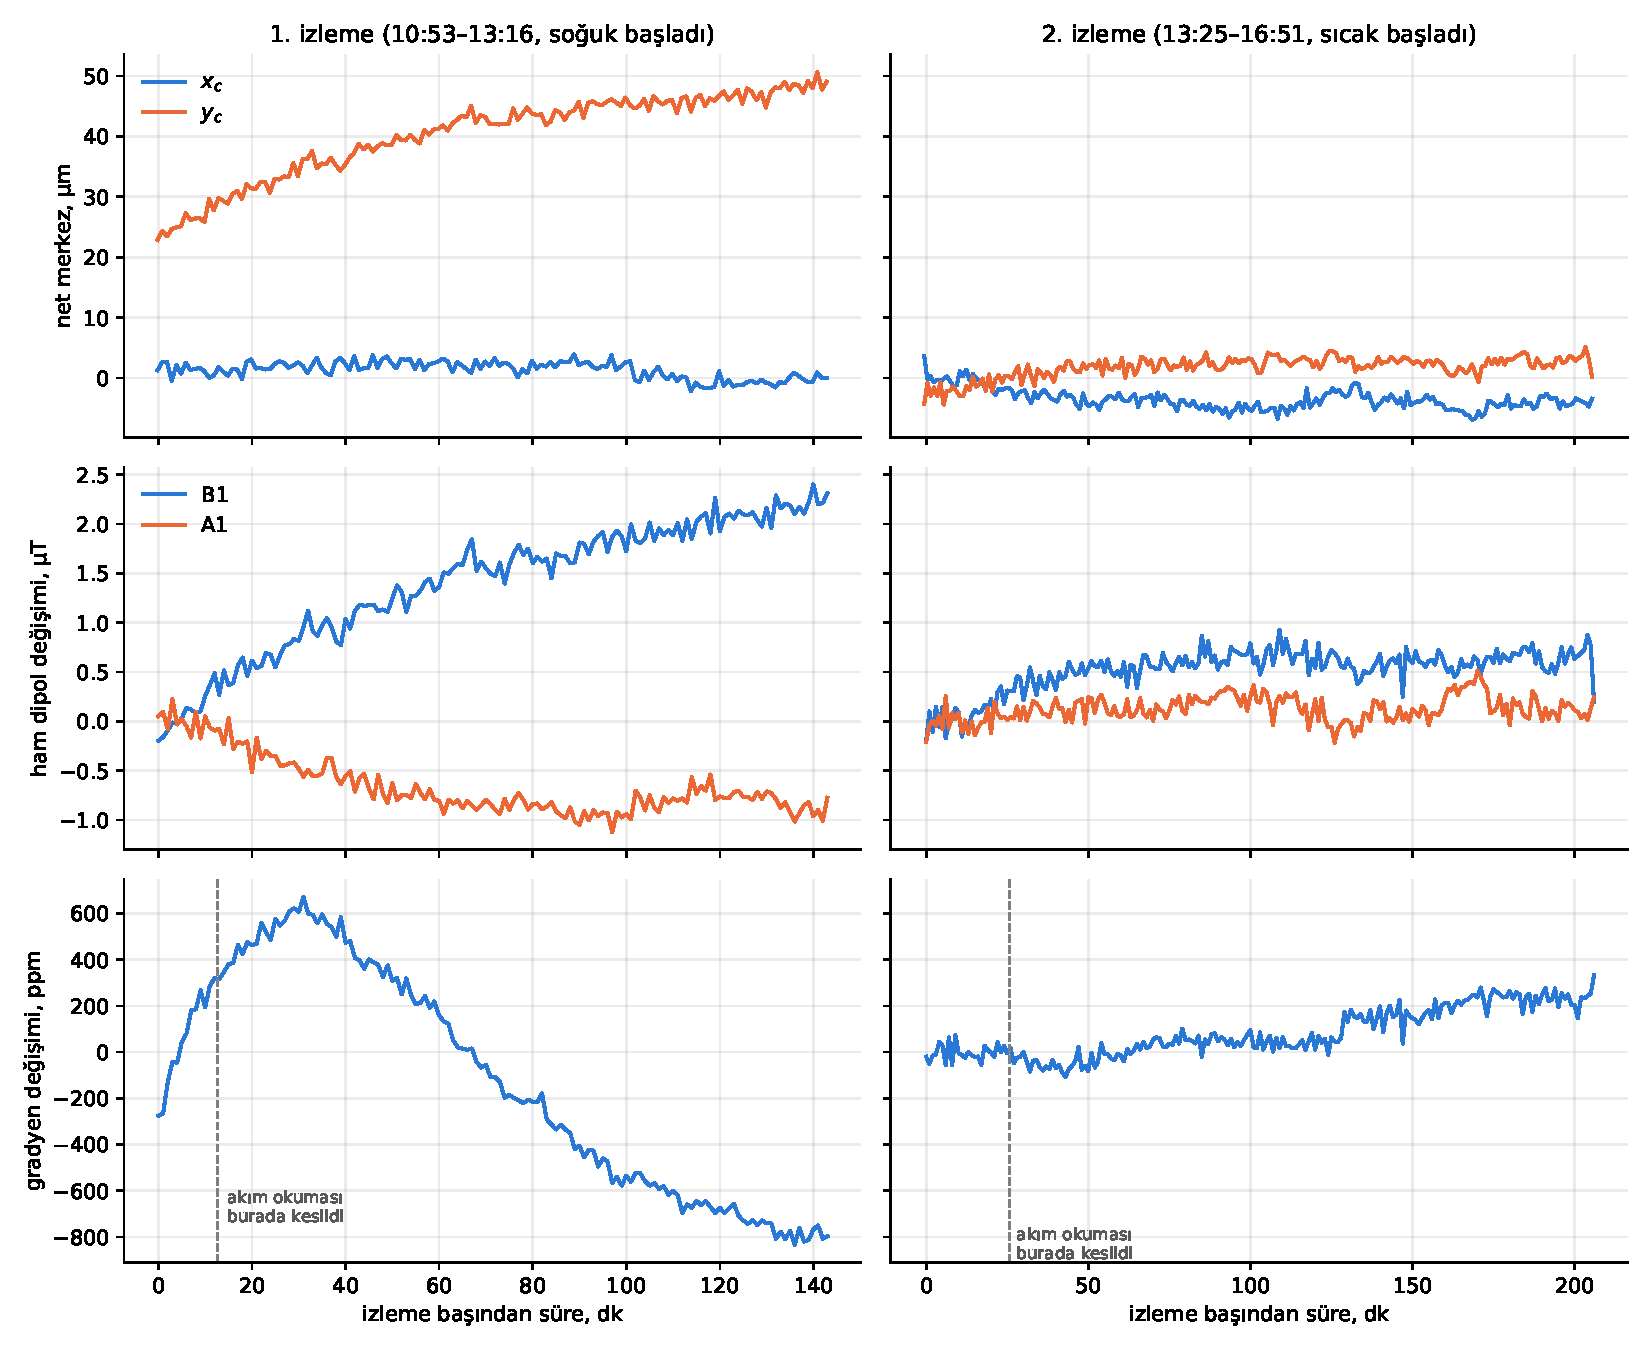
\includegraphics[width=\linewidth]{sekil1_izleme.pdf}
\caption{Üst sıra: net merkez (denklem~\ref{eq:merkez}), 1 dakikalık ortalamalar. Orta sıra: arka plan
çıkarılmamış ham dipol, ilk 10 dakikaya göre değişim. Alt sıra: ölçülen gradyenin ilk 10 dakikaya göre
değişimi (milyonda bir, ppm). Kesikli çizgi, güç kaynağı akımlarının okunamamaya başladığı an.}
\label{fig:izleme}
\end{figure}

\begin{table}[h]
\centering\small
\begin{tabular}{lrrrrr}
\toprule
 & ilk 15 dk & son 15 dk & doğrusal eğim & üstel $\tau$ & ardışık kayıt \\
 & (µm) & (µm) & (µm/saat) & (dk) & gürültüsü (µm) \\
\midrule
1. izleme, $x_c$ & $+1.4$ & $-0.3$ & $-1.1 \pm 0.1$ & -- & 2.8 \\
1. izleme, $y_c$ & $+26.3$ & $+48.0$ & $+9.4 \pm 0.2$ & $55 \pm 4$ & 4.2 \\
2. izleme, $x_c$ & $0.0$ & $-3.9$ & $-0.9 \pm 0.1$ & $26 \pm 3$ & 2.7 \\
2. izleme, $y_c$ & $-2.2$ & $+3.0$ & $+1.1 \pm 0.1$ & $30 \pm 5$ & 3.5 \\
\bottomrule
\end{tabular}
\caption{Net merkezin özeti. ``Üstel $\tau$'': $y(t) = a + b\,(1 - e^{-t/\tau})$ biçiminde bir ısınma eğrisi
uydurulduğunda bulunan zaman sabiti. 1. izlemenin $x_c$'sinde bu eğri anlamlı bir sonuç vermedi.
``Ardışık kayıt gürültüsü'' art arda gelen iki 10~s'lik kaydın farkından hesaplanır ve yavaş kaymadan
etkilenmez. Eğim belirsizlikleri yalnız istatistikseldir.}
\label{tab:merkez}
\end{table}

\subsection{Birinci izleme: y yönünde yavaşlayan bir kayma}
Şekil~\ref{fig:izleme}'nin sol üst grafiğinde $y_c$ 23~µm'den başlayıp 2.4 saatte yaklaşık 48~µm'ye
çıkıyor. $x_c$ ise yalnızca birkaç µm oynuyor \olc. Kayma düz bir doğru değil, yavaşlıyor: ilk 40 dakikada
yaklaşık 13~µm, son 40 dakikada yaklaşık 4~µm. Isınma eğrisi uydurulunca $\tau = 55 \pm 4$~dakika ve
toplam genlik $27$~µm çıkıyor. Bu eğriye göre kaymanın sonuna yaklaşılmıştı.

Kaymayı ham dipolde de görebiliyoruz (orta sıra). B1 2.4 saatte $-13.43$'ten $-11.38$~µT'ye çıktı, yani
2.05~µT değişti. Bölüm~1.1'deki oranla bu $2.05 \times 9.83 \approx 20$~µm eder. Bu değer tablodaki
22~µm'lik kaymaya çok yakın; yani merkez kayması gerçekten bobinin gördüğü dipoldeki değişimden geliyor
\olc. (B1'in $y_c$'yi değiştirmesi, mıknatısın bobine göre dönük durmasından kaynaklanır: $C_2$'nin skew
kısmı normal kısmından büyük, $C_2 \approx (1.15 + 2.27\,i)$~mT.)

\subsection{İkinci izleme: kararlı}
İkinci izlemede merkez 3.4 saat boyunca $\pm 5$~µm içinde kaldı (sağ üst grafik). Doğrusal eğimler saatte
yaklaşık 1~µm \olc. İlk 30 dakikada x ve y'de birkaç µm'lik bir oturma var (üstel $\tau \approx
26$--$30$~dk, genlik 6~µm), sonrası düz. Ham dipol de 0.6~µT'nin altında değişti.

Ardışık kayıt gürültüsü (2.7--3.5~µm) 12 Kasım'dakiyle (2.1--2.4~µm) aynı düzeyde. Yani ölçümün kısa
süreli çözünürlüğü değişmedi; değişen, merkezin kendi hareketi.

\subsection{12 Kasım ile karşılaştırma}
12 Kasım'da, bobin henüz sabitlenmemişken, merkez x yönünde saatte 30--36~µm kaymış ve iki saatlik soğumadan
sonra geri dönmemişti \olc{} (12 Kasım raporu). O rapor bunun mekanik bir sünmeden, yani bobinin ya da milin
mıknatısa göre yavaşça yer değiştirmesinden gelebileceğini öne sürmüştü \hip. Bugünkü ikinci izlemede kayma
30 kat daha küçük. Bu, eski kaymanın büyük kısmının bobinle mıknatıs arasındaki göreli hareketten geldiği
fikrini güçlendiriyor \yor. Kesin bir kanıt değil: arada başka şeyler de değişmiş olabilir (ortam alanının
yönü bile farklı, çünkü düzenek yeniden kuruldu).

\section{Kaymanın nedeni: ısınma}
\label{sec:isinma}

Bu bölümde birinci izlemedeki kaymanın ısınmadan geldiğini düşündüren kanıtları topluyoruz.

\subsection{Ortam alanı değişmedi}
Merkezleme sırasında her akımlı ölçümden önce bir akımsız arka plan ölçülür; her merkezlemede 15 tane.
Ortalamaları şöyle \olc:
\begin{center}\small
\begin{tabular}{lrr}
\toprule
 & B1 (µT) & A1 (µT) \\
\midrule
1. merkezleme (10:46--10:52) & $-15.65 \pm 0.81$ & $28.74 \pm 0.67$ \\
2. merkezleme (13:19--13:25) & $-15.93 \pm 0.74$ & $28.52 \pm 0.52$ \\
\bottomrule
\end{tabular}
\end{center}
($\pm$ işareti tek bir ölçümün saçılımıdır.) İki ortalama arasındaki fark 0.3~µT'den küçük. Oysa birinci
izlemede akımlı dipol 2~µT değişti. Demek ki bu değişim ortamdan değil, akım açıkken mıknatısın kendisinden
ya da bobinin mıknatısa göre konumundan geliyor \yor.

\subsection{Bobinler ısındı}
Güç kaynakları merkezleme sırasında hem akımı hem gerilimi ölçüyor. Bunların oranı, $R = U/I$, kuadrupol
bobinlerinin direncidir. Bakırın direnci sıcaklıkla artar:
\begin{equation}
  \frac{R(T)}{R(T_0)} = 1 + \alpha\,(T - T_0), \qquad \alpha = 0.00393\ \text{K}^{-1}
\end{equation}
Burada $\alpha$ bakırın direnç sıcaklık katsayısıdır: direnç her kelvinde yaklaşık binde 4 artar.

Dört bobinin ortalama direnci 1. merkezlemenin başında (10:46) 0.7116~Ω, 2. merkezlemenin başında (13:19)
0.7739~Ω idi \olc. Artış
\[
  \frac{0.7739}{0.7116} - 1 = 0.088 \quad (\%8.8),\qquad
  \Delta T = \frac{0.088}{0.00393} \approx 22\ \text{K}.
\]
Bu, bobinlerin ortalama sıcaklığının yaklaşık 22~K arttığı anlamına gelir \yor{} (gerilim kaynak
uçlarında ölçülüyorsa kablolar da bu dirence dahildir; o durumda sayı biraz farklı olur).

İki merkezlemenin içindeki eğilim de anlamlı. Birincide direnç 6 dakikada 0.7116'dan 0.7140~Ω'a
\emph{arttı}: mıknatıs soğuktu ve ısınıyordu. İkincide 0.7739'dan 0.7709~Ω'a \emph{azaldı}: mıknatıs sıcaktı,
merkezlemedeki akımsız adımlar ve öncesindeki birkaç dakikalık ara yüzünden biraz soğuyordu \olc.

\subsection{Yorum}
Bu üç gözlem birlikte tutarlı bir tablo veriyor \yor:
\begin{itemize}
\item Birinci izleme soğuk mıknatısla başladı; mıknatıs ısındıkça merkez kaydı ve kayma, ısınma durulurken
yavaşladı ($\tau \approx 55$~dk).
\item İkinci izleme, ısınmış mıknatısla başladı ve neredeyse hiç kaymadı.
\end{itemize}
Isınmanın merkezi nasıl kaydırdığını bu veriden ayıramıyoruz. Adaylar: (a) bobinlerin ya da demirin ısıl
genleşmesiyle manyetik merkezin yer değiştirmesi, (b) dört bobinin farklı ısınması, (c) bobin taşıyıcısının
mıknatısa göre kayması \hip. [v2] (d) Güç kaynaklarının kendi ısınmasıyla gerçek akımların kayması da aynı
güçte bir aday. İlk sürümde bunu gradyen gözlemiyle dışladığımızı yazmıştık; bu çıkarım geçerli değil
(Bölüm~\ref{sec:kaynak}).

\subsection{Gradyenin değişimi}
Ölçülen gradyen birinci izlemede ilk 31 dakikada 671~ppm arttı, sonra azalarak sonda başlangıcın
793~ppm altına indi (Şekil~\ref{fig:izleme}, sol alt) \olc. Akımlar sabitken gradyenin \%0.15 değişmesi
dikkat çekici. Güç kaynağı akımlarının okunabildiği ilk 12.7 dakikada gradyen 586~ppm arttı; aynı sürede
dört akımın toplamı yalnızca 14~ppm değişti \olc.

[v2] İlk sürümde buradan ``ilk artış güç kaynaklarından gelmiyor'' sonucunu çıkarmıştık. Bu çıkarım
zayıf: kaynağın okuduğu akım, akımı ayarlamakta kullandığı aynı iç ölçüm direncinden geliyor. O direnç
ısınıp değişirse gerçek akım değişir ama okuma değişmez (Bölüm~\ref{sec:kaynak}). Kaynağın teknik
özellikleri 30 dakikada \%0.02 + 2~mA, yani 9.5~A'de yaklaşık 4~mA (420~ppm) kaymaya izin veriyor; 586~ppm bu
büyüklükte. Dolayısıyla gradyendeki değişim ya kaynaklardan ya da mıknatıs ve ölçüm bobininin ısınmasından
gelebilir; eldeki veriyle ayıramıyoruz \yor.

Isınma tarafında olası bir açıklama şu \hip: Ölçüm bobini mıknatısın içinde olduğu için çabuk ısınır, yarıçapı büyür ve
duyarlılığı artar. Bu, gradyeni olduğundan büyük gösterir (hızlı artış). Demir ve bobin gövdesi ise
yavaş ısınır; aralık (gap) genişledikçe gerçek gradyen azalır (yavaş düşüş). Bunu doğrulamak için bobinin
ve mıknatısın sıcaklığını doğrudan ölçmek gerekir. İkinci izlemede gradyen 3.4 saatte yalnızca 234~ppm
değişti.

\section{Aksaklıklar}
\label{sec:aksak}

Bu bölüm ölçüm sırasında görülen sorunları ve yapılan düzeltmeleri anlatıyor.

\subsection{Motorun durması: yazılım hatası}
Günlükte son ölçüm 16:51:13'te yazılmış. Hız 8.004~Hz ve uydurma artığı normal. Günlükte ``hız tolerans
dışında'' satırı yok; motor yavaşlasaydı bu satır çıkardı. 16:51:15'te ölçüm döngüsü
\kod{IndexError('index -1 is out of bounds for axis 0 with size 0')} hatası verdi. Döngünün hata yakalayıcısı
(\kod{merkezleme\_penceresi.py}, \kod{\_tick}) her beklenmeyen hatada motoru güvenle durduruyor. Motor
16:51:20'de durdu \olc. Yani motor kendiliğinden durmadı; ölçüm hatası yüzünden program durdurdu.

Hatanın tam yerini kayıtlardan bulamıyoruz, çünkü yakalayıcı hata iletisini günlüğe yazıyor ama nerede
oluştuğunu (traceback) yazmıyordu. İletiye göre boş bir dizinin son elemanı istenmiş. En güçlü aday, ölçüm
hesabında tam tur sayan \kod{\_tam\_tur} işlevi: açı düzeltmesi ölçüm penceresini boşaltırsa bu işlev boş
dizinin son elemanını ister. Yapay olarak boşaltılmış bir pencereyle denediğimizde, düzeltmeden önceki kod
17 Kasım'daki iletinin \emph{birebir aynısını} verdi \olc. Gerçek ölçümde pencerenin neden boşaldığını
bilmiyoruz \hip.

\textbf{Düzeltmeler:} (1) Ölçüm hesabı, kırpmalardan sonra pencerede 100 örnekten az kalırsa bunu
anlaşılır bir \kod{ValueError} ile reddediyor. Ölçüm döngüsü bu hatayı zaten yakalıyor: o ölçüm atlanır,
günlüğe ``Ölçüm hesaplanamadı'' yazılır, motor dönmeye devam eder. (2) Döngünün hata yakalayıcısı artık her
beklenmeyen hatada hatanın yerini (traceback'in son satırlarını) günlüğe yazıyor. Böylece başka bir yerden
gelen bir hata da bir sonraki seferde bulunabilir. İkisi için de test eklendi.

\subsection{Güç kaynağı akımları okunamadı}
İzleme dosyalarında dört akım sütunu birinci izlemede 11:05'ten (12.7~dk), ikinci izlemede 13:51'den
(25.8~dk) sonra hep NaN \olc. Akımları okuyan iş parçacığı her hatayı sessizce yutup NaN yazıyordu; bu yüzden
hatanın ne olduğu günlükte yok. Akımların kendisi açık kaldı: gradyen izlemenin sonuna kadar sürdü. Bu
aksaklık yüzünden güç kaynağı kaymasını bütün izleme boyunca ölçemedik.

Okunabildiği sürede okunan akımlar çok kararlıydı: 12.7 dakikada en çok 0.2~mA değişti (milyonda 21) \olc.
[v2] Bu, okumanın kararlı olduğunu gösterir; gerçek akımın kararlı olduğunu göstermez (Bölüm~\ref{sec:kaynak}).

\textbf{Düzeltme:} okuma hatası artık günlüğe yazılıyor: ilk hata iletisiyle birlikte, sonra her 60
başarısız okumada bir özet, okuma düzelince de bir satır. Akımlar hâlâ NaN olarak kaydediliyor ve izleme
sürüyor; ama bir sonraki uzun ölçümde okumanın neden kesildiği günlükten anlaşılacak.

\subsection{[v2] Güç kaynağının okuduğu akım ne kadar güvenilir?}
\label{sec:kaynak}

12 Kasım'daki ölçümlerin sonuna doğru, bilgisayarın güç kaynaklarından okuduğu akım ile kaynakların ön
panelinde görünen akım arasında mA düzeyinde farklar görüldü. Bu bölümde bunun ne anlama geldiğini, kaynağın
teknik özellikleri ve kayıtlardaki okumalarla açıklıyoruz. Ön panel değerleri kaydedilmediği için panel ile
bilgisayarı doğrudan karşılaştıramıyoruz.

\textbf{Teknik özellikler} \olc{} (ITECH IT-M3200 veri sayfası, IT-M3233, 10~A aralığı, 23$\pm$5~°C, 12 ay):
\begin{center}\small
\begin{tabular}{lrr}
\toprule
 & tanım & 9.5~A'de \\
\midrule
Ayar doğruluğu & $\pm$(\%0.05 + 5~mA) & $\pm$9.8~mA \\
Okuma doğruluğu & $\pm$(\%0.05 + 5~mA) & $\pm$9.8~mA \\
Ayar ve okuma çözünürlüğü & 1~mA & \\
Ayar kararlılığı, 30~dk & \%0.02 + 2~mA & 3.9~mA \\
Ayar kararlılığı, 8~saat & \%0.05 + 3~mA & 7.8~mA \\
Okuma kararlılığı, 30~dk & \%0.02 + 3~mA & 4.9~mA \\
Okuma kararlılığı, 8~saat & \%0.05 + 3~mA & 7.8~mA \\
\bottomrule
\end{tabular}
\end{center}
``\%0.05 + 5~mA'' şu demek: izin verilen hata, akımın binde yarısına 5~mA eklenerek bulunur. 9.5~A için
$9.5 \times 0.0005 = 4.75$~mA, artı 5~mA, toplam yaklaşık 9.8~mA.

Bundan iki sonuç çıkıyor \yor. Birincisi, kaynak \kod{MEAS:CURR?} sorusuna beş ondalıklı bir sayıyla
(ör. 9.82907) yanıt veriyor; kayıtlarda okumaların 0.01~mA adımlarla değiştiği görülüyor \olc. Ama üretici
yalnızca 1~mA çözünürlüğü garanti ediyor; son iki hane anlamlı değil. İkincisi, ön panel ile bilgisayar
arasında mA düzeyinde fark görmek beklenen bir şey: panel değeri yuvarlar, ayrıca kendi okuma ve ortalama
zamanlaması vardır. Bu fark teknik özelliklerin çok içinde.

\textbf{Kayıtlardaki okumalar.} Okunan akım ile ayar değeri arasındaki fark (mA) \olc:
\begin{center}\small
\begin{tabular}{lrrrr}
\toprule
 & bobin 1 & bobin 2 & bobin 3 & bobin 4 \\
\midrule
17 Kasım, 1. merkezleme (soğuk) & $-0.01$ & $-0.13$ & $-0.11$ & $-0.03$ \\
17 Kasım, 2. merkezleme (sıcak) & $+0.47$ & $+0.36$ & $-0.07$ & $+0.25$ \\
12 Kasım, 1. akımlı bölüm, ilk 10 kayıt & $+0.27$ & $+0.21$ & $-0.29$ & $+0.21$ \\
12 Kasım, 1. akımlı bölüm, son 10 kayıt & $+0.63$ & $+0.54$ & $-0.26$ & $+0.41$ \\
12 Kasım, 1. akımlı bölüm, eğim (mA/saat) & $+0.26$ & $+0.24$ & $+0.03$ & $+0.12$ \\
\bottomrule
\end{tabular}
\end{center}
Fark, kaynaklar ısındıkça hep aynı üç kaynakta (bobin 1, 2, 4) ve aynı yönde açılıyor; bobin 3'ün kaynağı
hemen hiç değişmiyor. Fark her durumda 1~mA'in altında, teknik özelliklerin çok içinde. Akım sıfırken iki kaynak
0.1--0.35~mA gösteriyor; bu daha önce bilinen kalıntı. Bu farkın, kaynağın içindeki ayar devresi ile okuma
devresinin ısınmayla birbirinden biraz ayrılmasından geldiğini düşünüyoruz \hip.

\textbf{Okuma neden gerçek akımın kararlılığını kanıtlamıyor?} Sabit akım kipinde kaynak, çıkış akımını
içindeki bir ölçüm direncinden (şönt) geçirir, üstündeki gerilimi ölçer ve ayar değerine eşitlemeye çalışır.
\kod{MEAS:CURR?} de aynı şöntün gerilimini okur. Şönt ısınıp direnci, örneğin, milyonda 300 değişirse kaynak
gerçek akımı milyonda 300 kaydırır, ama okuma ayar değerini göstermeye devam eder: hata, ayarlamada da
okumada da aynıdır ve birbirini götürür. Bu yüzden ``okunan akım sabitti'' cümlesi yalnızca kaynağın kendi
iç tutarlılığını anlatır \yor.

\textbf{Bu ölçüm için ne kadar önemli?} 17 Kasım kalibrasyonuna göre bir bobindeki 1~mA'lik değişim merkezi
en çok 2.2~µm kaydırıyor \olc. Kaynağın 8 saatlik kararlılık sınırı olan 7.8~mA, tek bir bobinde merkezde
yaklaşık $7.8 \times 2.2 \approx 17$~µm demek. Bu, birinci izlemedeki 22~µm'lik kaymayla aynı büyüklükte.
Yani o kaymanın bir kısmı kaynaklardan da gelebilir \hip. Öte yandan merkezleme kaynağın okumasına değil,
dönen bobinin manyetik ölçümüne dayanıyor. İkinci izlemede merkezin 3.4 saat $\pm 5$~µm içinde kalması,
sıcak düzende gerçek akımlardaki dengesizliğin aynı süre boyunca yaklaşık $\pm 2$~mA içinde kaldığını
gösteriyor \yor.

\textbf{Nasıl ayırt edilir?} Gerçek akımı kaynaktan bağımsız ölçmek gerekir: en az bir bobin devresine hassas
bir şönt (düşük sıcaklık katsayılı) ve multimetre, ya da akım dönüştürücü (DCCT) koyup soğuk başlayan bir
izleme yapmak. Merkez kayarken bağımsız ölçülen akım da kayıyorsa neden kaynaktır; kaymıyorsa mıknatıstır.

\subsection{Merkezleme 5~µm toleransa yakınsamadı}
\label{sec:yakinsama}
Her iki merkezlemede de son üç yineleme y yönünde salındı \olc:
\begin{center}\small
\begin{tabular}{lrrr}
\toprule
 & yineleme 3 & yineleme 4 & yineleme 5 \\
\midrule
1. merkezleme $(x, y)$, µm & $(-0.9,\ 19.6)$ & $(1.0,\ -26.0)$ & $(5.9,\ 23.2)$ \\
2. merkezleme $(x, y)$, µm & $(4.5,\ 23.1)$ & $(-2.6,\ -15.2)$ & $(10.3,\ 3.5)$ \\
\bottomrule
\end{tabular}
\end{center}
Merkezleme 5 yinelemede durdu ve doğrulama uyarısı onaylanarak bitirildi. Birinci izleme bu yüzden 23~µm'den
başladı. Salınım (30--50~µm) tek ölçüm gürültüsünden (3--4~µm) çok büyük. Kalibrasyon dosyası da kendini
``şüpheli'' olarak işaretlemiş (monopol sızıntısı, y'de doğrusal olmayan yanıt) \olc. Düzeltme adımlarının
fazla büyük olması (aşma) ya da kalibrasyonun ısınan mıknatısta alınması olası nedenler \hip. Bu ayrıca
incelenmeli; bu raporun kapsamında düzeltilmedi.

\subsection{Tek arka plan ölçümünün gürültüsü}
Tek bir akımsız arka plan ölçümünün saçılımı 0.5--0.8~µT. Bölüm~1.1'deki orana göre bu, merkezde 5--8~µm
belirsizlik demek. Merkezleme ve izleme yalnızca \emph{son} arka planı kullanıyordu. Bugünkü iki izlemede son
arka planın ortalamadan farkı merkezi en çok yaklaşık 5~µm etkiledi \olc.

\textbf{Düzeltme:} izleme artık arka plan olarak merkezlemedeki son beş akımsız ölçümün ortalamasını
kullanıyor (\kod{birlesik.py}, \kod{ARKA\_PLAN\_ORTALAMA\_SAYISI}). Merkezlemede her noktada arka plan
alındığı için bunlar son yaklaşık 2 dakikaya aittir; ortam bu sürede değişmediği için ortalama doğruluğu
bozmadan gürültüyü azaltır: beş ölçümün ortalamasında saçılım $0.8/\sqrt{5} \approx 0.36$~µT, yani
yaklaşık 3.5~µm. Merkezlemenin kendi hesabı değiştirilmedi; orada her noktada taze arka plan kullanılması
bilerek seçilmiş bir yöntem. Bölüm~\ref{sec:yakinsama}'teki salınım da arka plan gürültüsünden gelmiyor: yinelemeleri
ortalama arka planla yeniden hesaplayınca salınım sürüyor \olc.

\subsection{Küçük notlar}
Günlükte 11:46'dan sonra 485 ``okuma saati sıçraması'' uyarısı var (saatte yaklaşık 100). Eşiğin hemen
üstünde (0.60--0.68 örnek) ve sonuçlarda bir iz görünmüyor \olc. 15:52'deki ``dipol saçılımı 4.2~µT'' uyarısı
tek bir ölçümden geliyor; o dakikanın ortalaması etkilenmedi \olc.

\section{Sonuç ve öneriler}

Bobin kuadrupole sabitlendikten sonra merkez, ısınmış mıknatısta saatte yaklaşık 1~µm kayıyor. Bu, 12
Kasım'daki 30~µm/saatin yanında büyük bir iyileşme ve 5~µm'lik merkezleme hedefi için yeterli. Soğuk
düzende ise ilk 1--2 saatte 20--25~µm'lik ısınmaya bağlı bir kayma var. [v2] Bu kaymanın mıknatısın mı
yoksa güç kaynaklarının mı ısınmasından geldiğini eldeki veriyle ayıramıyoruz.

Önerilerimiz:
\begin{enumerate}
\item \textbf{Merkezlemeden önce mıknatısı ısıtmak:} akımları yaklaşık 2 saat ($\approx 2\tau$) açık
tutmak ya da merkezlemeyi ısıl dengeye gelince tekrarlamak.
\item \textbf{Sıcaklığı ölçmek:} kuadrupol bobinlerine ve ölçüm bobini yakınına birer sıcaklık sensörü
koymak. Gradyenin ve merkezin ısınmaya nasıl bağlı olduğu ancak böyle ayrılabilir.
\item \textbf{[v2] Gerçek akımı bağımsız ölçmek:} en az bir bobin devresinde hassas şönt ve multimetre ya da
DCCT ile soğuk başlayan bir izleme yapmak. Kaymanın kaynaktan mı mıknatıstan mı geldiğini ancak bu ayırır.
Ön panel değerleri de bu sırada saatleriyle not edilirse bilgisayarın okumasıyla karşılaştırılabilir.
\item \textbf{Merkezleme yakınsamasını incelemek:} son yinelemelerdeki salınımın nedenini bulmak
(adım küçültme, birkaç ölçümün ortalaması, ısınmış mıknatısta yeni kalibrasyon).
\item \textbf{Bir sonraki uzun ölçümde akım okumasını izlemek:} yeni günlük satırları, akım okumasının neden
kesildiğini gösterecek.
\end{enumerate}

\end{document}
